% Architecture Diagram for Context Tracker
% Compile with: pdflatex architecture_diagram.tex
%
% Required packages: tikz, xcolor

\documentclass[tikz,border=10pt]{standalone}
\usepackage{tikz}
\usepackage{xcolor}
\usepackage{amsmath}
\usepackage{amssymb}

\usetikzlibrary{
    shapes.geometric,
    shapes.misc,
    arrows.meta,
    positioning,
    calc,
    fit,
    backgrounds,
    matrix,
    decorations.pathreplacing
}

% Define colors (academic paper style)
\definecolor{inputcolor}{RGB}{255, 235, 180}      % Light yellow
\definecolor{decodercolor}{RGB}{255, 200, 100}    % Orange/yellow
\definecolor{encodercolor}{RGB}{180, 220, 180}    % Light green
\definecolor{tokencolor}{RGB}{180, 200, 255}      % Light blue
\definecolor{headcolor}{RGB}{255, 180, 180}       % Light red/pink
\definecolor{modulecolor}{RGB}{200, 255, 200}     % Light green box
\definecolor{matrixhigh}{RGB}{180, 50, 50}        % Dark red for matrix
\definecolor{matrixlow}{RGB}{255, 220, 220}       % Light pink for matrix

\begin{document}

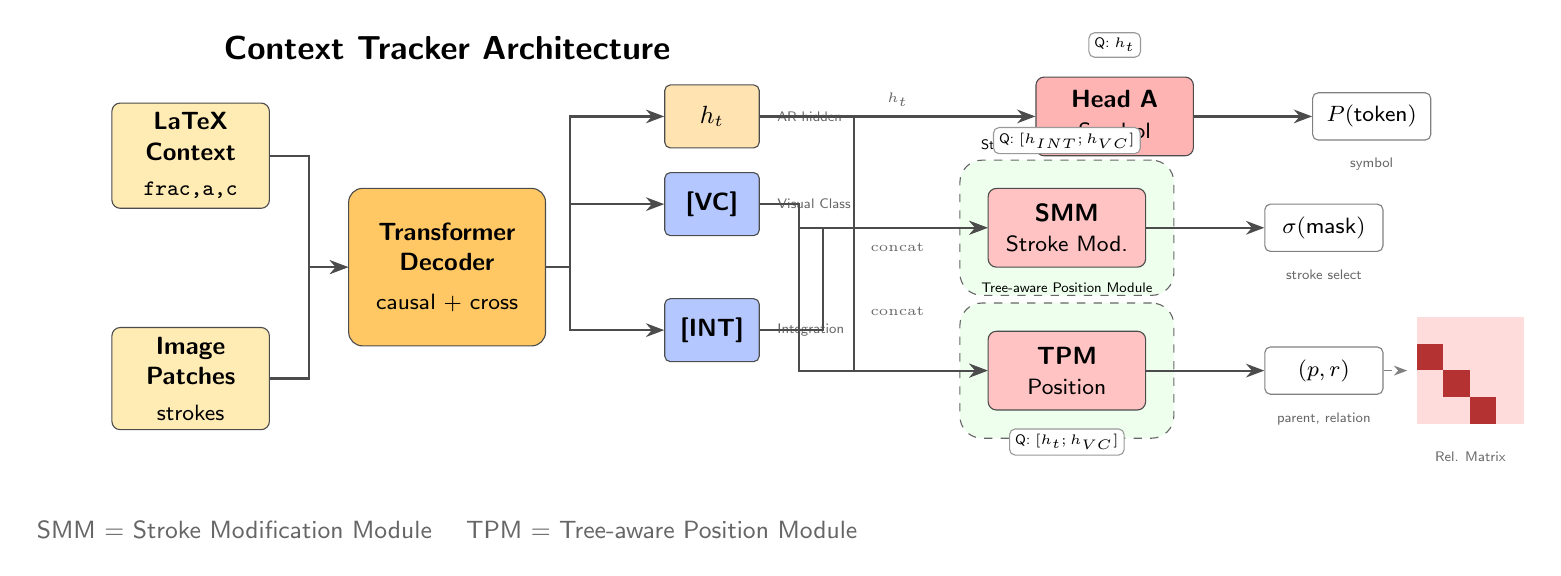
\begin{tikzpicture}[
    % Node styles
    input/.style={
        rectangle, 
        draw=black!70, 
        fill=inputcolor, 
        rounded corners=3pt,
        minimum width=2cm, 
        minimum height=1.2cm,
        font=\small\sffamily,
        align=center
    },
    decoder/.style={
        rectangle, 
        draw=black!70, 
        fill=decodercolor, 
        rounded corners=5pt,
        minimum width=2.5cm, 
        minimum height=2cm,
        font=\small\sffamily,
        align=center
    },
    encoder/.style={
        rectangle, 
        draw=black!70, 
        fill=encodercolor, 
        rounded corners=5pt,
        minimum width=2cm, 
        minimum height=1.5cm,
        font=\small\sffamily,
        align=center
    },
    token/.style={
        rectangle, 
        draw=black!70, 
        fill=tokencolor, 
        rounded corners=2pt,
        minimum width=1.2cm, 
        minimum height=0.8cm,
        font=\small\sffamily
    },
    head/.style={
        rectangle, 
        draw=black!70, 
        fill=headcolor, 
        rounded corners=3pt,
        minimum width=2cm, 
        minimum height=1cm,
        font=\small\sffamily,
        align=center
    },
    module/.style={
        rectangle, 
        draw=black!60, 
        dashed,
        fill=modulecolor!30, 
        rounded corners=8pt,
        inner sep=10pt
    },
    output/.style={
        rectangle, 
        draw=black!50, 
        fill=white, 
        rounded corners=2pt,
        minimum width=1.5cm, 
        minimum height=0.6cm,
        font=\footnotesize\sffamily
    },
    arrow/.style={
        ->,
        >=Stealth,
        thick,
        black!70
    },
    dashedarrow/.style={
        ->,
        >=Stealth,
        dashed,
        black!50
    }
]

% ============================================
% INPUT SECTION
% ============================================

% LaTeX Context Input
\node[input] (latex_input) {
    \textbf{LaTeX}\\
    \textbf{Context}\\[2pt]
    \footnotesize\texttt{frac,a,c}
};

% Image Patches Input
\node[input, below=1.5cm of latex_input] (image_input) {
    \textbf{Image}\\
    \textbf{Patches}\\[2pt]
    \footnotesize strokes
};

% ============================================
% TRANSFORMER DECODER
% ============================================

\node[decoder, right=2cm of $(latex_input)!0.5!(image_input)$] (transformer) {
    \textbf{Transformer}\\
    \textbf{Decoder}\\[3pt]
    \footnotesize causal + cross
};

% ============================================
% SPECIAL TOKENS
% ============================================

\node[token, right=1.5cm of transformer, yshift=0.8cm] (vc_token) {\textbf{[VC]}};
\node[token, right=1.5cm of transformer, yshift=-0.8cm] (int_token) {\textbf{[INT]}};

% Token labels
\node[right=0.1cm of vc_token, font=\tiny\sffamily, text=black!60] {Visual Class};
\node[right=0.1cm of int_token, font=\tiny\sffamily, text=black!60] {Integration};

% AR hidden state
\node[token, above=0.3cm of vc_token, fill=decodercolor!50] (ht_token) {$h_t$};
\node[right=0.1cm of ht_token, font=\tiny\sffamily, text=black!60] {AR hidden};

% ============================================
% THREE HEADS
% ============================================

% Head A - Symbol
\node[head, right=3.5cm of ht_token] (head_a) {
    \textbf{Head A}\\
    \footnotesize Symbol
};

% SMM - Stroke Modification Module
\node[head, right=3.5cm of $(vc_token)!0.5!(int_token)$, yshift=0.5cm, fill=headcolor!80] (smm) {
    \textbf{SMM}\\
    \footnotesize Stroke Mod.
};

% TPM - Tree-aware Position Module  
\node[head, below=0.8cm of smm, fill=headcolor!80] (tpm) {
    \textbf{TPM}\\
    \footnotesize Position
};

% ============================================
% MODULE BOXES (dashed)
% ============================================

% SMM Module Box
\begin{scope}[on background layer]
    \node[module, fit=(smm), label={[font=\tiny\sffamily]above:Stroke Modification Module}] (smm_box) {};
\end{scope}

% TPM Module Box
\begin{scope}[on background layer]
    \node[module, fit=(tpm), label={[font=\tiny\sffamily]above:Tree-aware Position Module}] (tpm_box) {};
\end{scope}

% ============================================
% OUTPUTS
% ============================================

\node[output, right=1.5cm of head_a] (out_symbol) {\footnotesize $P(\text{token})$};
\node[output, right=1.5cm of smm] (out_stroke) {\footnotesize $\sigma(\text{mask})$};
\node[output, right=1.5cm of tpm] (out_pos) {\footnotesize $(p, r)$};

% Output labels
\node[below=0.1cm of out_symbol, font=\tiny\sffamily, text=black!60] {symbol};
\node[below=0.1cm of out_stroke, font=\tiny\sffamily, text=black!60] {stroke select};
\node[below=0.1cm of out_pos, font=\tiny\sffamily, text=black!60] {parent, relation};

% ============================================
% RELATIONSHIP MATRIX (for TPM)
% ============================================

\matrix[
    matrix of nodes,
    right=0.3cm of out_pos,
    nodes={minimum width=0.35cm, minimum height=0.35cm, font=\tiny},
    column sep=-\pgflinewidth,
    row sep=-\pgflinewidth,
] (relmatrix) {
    |[fill=matrixlow]| & |[fill=matrixlow]| & |[fill=matrixlow]| & |[fill=matrixlow]| \\
    |[fill=matrixhigh]| & |[fill=matrixlow]| & |[fill=matrixlow]| & |[fill=matrixlow]| \\
    |[fill=matrixlow]| & |[fill=matrixhigh]| & |[fill=matrixlow]| & |[fill=matrixlow]| \\
    |[fill=matrixlow]| & |[fill=matrixlow]| & |[fill=matrixhigh]| & |[fill=matrixlow]| \\
};
\node[below=0.1cm of relmatrix, font=\tiny\sffamily, text=black!60] {Rel. Matrix};

% ============================================
% ARROWS - Main flow
% ============================================

% Inputs to Transformer
\draw[arrow] (latex_input.east) -- ++(0.5,0) |- (transformer.west);
\draw[arrow] (image_input.east) -- ++(0.5,0) |- (transformer.west);

% Transformer to tokens
\draw[arrow] (transformer.east) -- ++(0.3,0) |- (vc_token.west);
\draw[arrow] (transformer.east) -- ++(0.3,0) |- (int_token.west);
\draw[arrow] (transformer.east) -- ++(0.3,0) |- (ht_token.west);

% ============================================
% ARROWS - Head connections with QUERY labels
% ============================================

% Head A: h_t -> symbol
\draw[arrow] (ht_token.east) -- node[above, font=\tiny, text=black!60] {$h_t$} (head_a.west);
\draw[arrow] (head_a.east) -- (out_symbol.west);

% SMM: concat(INT, VC) -> stroke
\draw[arrow] (int_token.east) -- ++(0.8,0) |- node[pos=0.25, above, font=\tiny, text=black!60] {} (smm.west);
\draw[arrow] (vc_token.east) -- ++(0.5,0) |- (smm.west);
\draw[arrow] (smm.east) -- (out_stroke.west);

% Add concat label for SMM
\node[font=\tiny, text=black!60] at ($(int_token.east)!0.5!(smm.west) + (0.3, 0.4)$) {concat};

% TPM: concat(h_t, VC) -> position
\draw[arrow] (ht_token.east) -- ++(1.2,0) |- (tpm.west);
\draw[arrow] (vc_token.east) -- ++(0.5,0) |- (tpm.west);
\draw[arrow] (tpm.east) -- (out_pos.west);
\draw[dashedarrow] (out_pos.east) -- (relmatrix.west);

% Add concat label for TPM
\node[font=\tiny, text=black!60] at ($(vc_token.east)!0.5!(tpm.west) + (0.3, -0.3)$) {concat};

% ============================================
% QUERY ANNOTATIONS
% ============================================

% Query boxes
\node[
    rectangle,
    draw=black!40,
    fill=white,
    rounded corners=2pt,
    font=\tiny\sffamily,
    inner sep=2pt
] at ($(head_a.north) + (0, 0.4)$) {Q: $h_t$};

\node[
    rectangle,
    draw=black!40,
    fill=white,
    rounded corners=2pt,
    font=\tiny\sffamily,
    inner sep=2pt
] at ($(smm.north) + (0, 0.6)$) {Q: $[h_{INT}; h_{VC}]$};

\node[
    rectangle,
    draw=black!40,
    fill=white,
    rounded corners=2pt,
    font=\tiny\sffamily,
    inner sep=2pt
] at ($(tpm.south) + (0, -0.4)$) {Q: $[h_t; h_{VC}]$};

% ============================================
% TITLE
% ============================================

\node[
    font=\large\bfseries\sffamily,
    above=1.5cm of transformer
] {Context Tracker Architecture};

\node[
    font=\small\sffamily,
    text=black!60,
    below=0.1cm of transformer,
    yshift=-2cm
] {SMM = Stroke Modification Module \quad TPM = Tree-aware Position Module};

\end{tikzpicture}

\end{document}

